% !TeX spellcheck = en_GB

\section{Modelling the Granule-Golgi Circuit}
\label{sec:cerebellum_golgi_granule}

As we discussed in the introduction, we would like to analyse in how far adding biological detail to a system influences its high-level function.
To this end, we focus on one specific part of the cerebellar microcircuit, namely the Granule-Golgi circuit, and test to what degree this circuit is capable of generating a temporal representation at five different levels of biological detail.
Below, we first describe these individual circuits, followed by a series of experiments in which we explore the performance of the individual networks.

\subsection{Levels of Biological Detail}
\label{sec:cerebellum_levels}

\begin{figure}
	\centering
	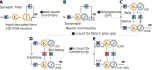
\includegraphics{media/chapters/05_cerebellum/network_types.pdf}%
	{\phantomsubcaption\label{fig:cerebellum_network_types_a}}%
	{\phantomsubcaption\label{fig:cerebellum_network_types_b}}%
	{\phantomsubcaption\label{fig:cerebellum_network_types_c}}%
	{\phantomsubcaption\label{fig:cerebellum_network_types_d}}%
	{\phantomsubcaption\label{fig:cerebellum_network_types_e}}%
	\caption[Network types used in the cerebellum experiments.]{Network types used in our experiments. \textbf{(A)} \enquote{Direct} implementation with an optimal integrator. \textbf{(B)} Using the synaptic filter of a single population of spiking neurons for temporal integration. \textbf{(C)} Inter-neuron population in the recurrent path. \textbf{(D)} Same as \emph{(C)}, but accounting for Dale's principle. \textbf{(E)} Same as \emph{(D)}, but with more detailed biological constraints (see text).}
	\label{fig:cerebellum_network_types}
\end{figure}

We discuss five models of increasing complexity (cf.~\Cref{fig:cerebellum_network_types}).
The first model is merely an abstract implementation of the delay network, the final model respects spatial connectivity constraints, tuning curves, and, to a degree, neurotransmitter time-constants.
In all cases, the input $u$ is received from an \NEF ensemble with $100$ spiking \LIF neurons representing the \PCN.

\subsubsection{Model A: \enquote{Direct} Implementation} 
For this model, we directly solve the differential equations describing the Legendre system (cf.~eq.~\ref{eqn:delay_network_lti}) by integration.
% TODO: Add correct reference to the delay network
That is, we have a single layer of \enquote{neurons} that are pure integrators.
Correspondingly, this model focuses on the high-level theory of what the system is computing.
We model the \PCN and the granule cells as neuron populations, but these are not responsible for generating the dynamics.

\subsubsection{Model B: Single Population}
In our second stage, we replace the integrators with an ensemble of $200$ \LIF neurons.
As we discussed in \Cref{sec:nef_representation}, these neurons form a distributed representation of the Legendre system state $\vec{m}$ using a population code (cf.~eq.~\ref{eqn:encoding}).
Maximum firing rates $a_\mathrm{max}$ are between \SIrange{50}{100}{\hertz}.
We solve for optimal input and recurrent connection weights that result in these desired tuning curves while implementing the equivalent calculation as in \emph{Model A} using the \NEF dynamics principle (\Cref{sec:nef_dynamics}).

\subsubsection{Model C: Inter-neurons}
As a next step, we separate the single layer of neurons into two populations corresponding to the Golgi and granule cells, reflecting the actual biology of the cerebellum.
This introduces two synaptic filters which need to be taken into account when solving for the connection weights that best approximate the Legendre system; we discussed this in \Cref{sec:lti_complex_networks}.
Furthermore, to at least approximate the fact that there are far fewer Golgi cells than granule cells, we use $20$ Golgi cells and $200$ granule cells.

\subsubsection{Model D: Inhibition and Excitation}
In the next step, we account for Dale's principle using the techniques described in \Cref{sec:nef_nonneg}.
We mark the graunle cells as purely excitatory, and the Golgi cells as purely inhibitory and decode the bias current from the pre-population.
Note that we assume---in contrast to the evidence presented in \Cref{fig:granule_jbias_distribution}---that the granule cells possess intrinsic biases and uniform $x$-intercepts; we discuss this in more detail below.

\subsubsection{Model E: Sparse connectivity and activities}
Finally, we constrain the neural connectivity and adjust the \PCN tuning.
The previous models used all-to-all connections, whereas we now only allow a subset of the connection weights to be non-zero.
This applies to both the input to the Granule-Golgi system and to the recurrent connections.

In particular, as is indicated in \Cref{fig:cerebellum_network_types_e}, we account for the granule cell convergence numbers by randomly selecting five \PCN and five Golgi cells as pre-neurons---this number is slightly larger than the number reported above, since, as we discuss in more detail in \Cref{sec:cerebellum_vary_parameters}, the number of pre-neurons places a strict upper limit on the connectivity. Given this extremely sparse connectivity, we increase the number of neurons in the simulation to \num{10000} granule and \num{100} Golgi cells, which is closer to the ratio observed in nature.

\begin{figure}
    \centering
    \includegraphics{media/chapters/05_cerebellum/spatial_constraints.pdf}
    \caption[Spatial connectivity constraints between the Golgi and granule cells]{Spatial connectivity constraints between the Golgi and granule cells.
    \textbf{(A)} Normalised connection probabilities $p_{ij}$ for $\sigma=0.25$. Note that the neuron locations are sampled from a Hilbert curve with additive random jitter. Correspondingly, neurons with similar (relative) indices tend to be closer together, resulting in the clearly visible diagonal.
    \textbf{(B)} Spatial organisation of the Golgi and granule cells. The background depicts the cumulative density of the Golgi to granule connection probability for a virtual Granule cell at each location; same colours as in \emph{(A)}.}
    \label{fig:spatial_constraints}
\end{figure}

\begin{figure}
	\centering
    \includegraphics{media/chapters/05_cerebellum/pcn_tuning.pdf}
    \caption[Granule cell EPSC distributions and PCN tuning curves]{Granule cell \EPSC distributions and \PCN tuning curves.
    \textbf{(A)} Empirical granule cell \EPSC rates (cf.~\cite{chadderton2004integration}, Figure 3C; rescaled from counts per bin to rates).
    Data are the mean over 16 trials.
    Black bar and shaded background correspond to stimulation of the animal's whiskers.
    Upper dashed line corresponds to the average spike rate with input (including the first bin after the input), lower dashed line to the average spike rate without input.
    \textbf{(B, C)} In our model, \PCN input via the mossy fibres is the only excitatory input to the granule cells. Setting the maximum firing rates to be uniformly distributed in $[25, 75]$ and the $x$-intercepts to be uniformly sampled from $(-0.15, 0.95)$ qualitatively results in a similar \EPSC distribution. Data are the mean over \num{10000} cells.
    }
    \label{fig:pcn_tuning}
\end{figure}

To account for spatially imposed connectivity constraints, we assign a location $\vec x$ in $[-1, 1]^2$ to each neuron.
This represents to a location on a small patch of the folded two-dimensional surface of the cerebellar cortex.
As is depicted in \Cref{fig:spatial_constraints}, the probability $p_{ij}$ of a post-neuron $i$ to receive a connection from a pre-neuron $j$ is proportional to $\exp \left(- \| \vec x_i - \vec x_j \|^2 / \sigma^{2} \right)$.%
\footnote{See \Cref{sec:nengo_bio_sparsity} for an overview of how these sparsity constraints can be specified in NengoBio.}

The input representation in the \PCN was made more temporally sparse by adjusting the $x$-intercepts (\Cref{sec:nef_representation}).
Data reported by \citet{chadderton2004integration} indicate that granule cell excitatory event rates---which are driven by \PCN activity---drop from an average of \SI{40}{\per\second} with a stimulus being present to only \SI{8.5}{\per\second} when there is no stimulus.
We adjusted the \PCN tuning curves to match these statistics in the final network (cf.~\Cref{fig:pcn_tuning}).


\subsection{Impact Of Biological Detail On Temporal Representations}

To explore the effect of adding biological detail to the Granule-Golgi circuit, we first take a look at the temporal representations generated by these systems.
We then analyse in how far we are able to decode delays from these representations, as is required for delay conditioning.

\subsubsection{Temporal Representations}

\begin{figure}
	\centering
    \includegraphics{media/chapters/05_cerebellum/basis_functions.pdf}%
    {\phantomsubcaption\label{fig:cerebellum_basis_functions_a}}%
    {\phantomsubcaption\label{fig:cerebellum_basis_functions_b}}%
    {\phantomsubcaption\label{fig:cerebellum_basis_functions_c}}%
    {\phantomsubcaption\label{fig:cerebellum_basis_functions_d}}%
    {\phantomsubcaption\label{fig:cerebellum_basis_functions_e}}%
    {\phantomsubcaption\label{fig:cerebellum_basis_functions_f}}%
    {\phantomsubcaption\label{fig:cerebellum_basis_functions_g}}%
    \vspace{0.5em}
    \caption[Temporal response of the Granule-Golgi networks]{
    	Temporal response of the Granule-Golgi networks for a rectangle input (black line).
    	All responses are centred and normalised.
    	\emph{Left:} Example identity decoding of the granule activities.
    	\emph{Centre and right:} Example singular value decomposition (\SVD) of the granule cell activities and the median normalised singular values over \num{100} trials. Error-bars indicate the 25th and 75th percentile.
    	\textbf{(A-E)} Data for the individual models discussed in this section.
    	\textbf{(F)} Network with a stable random feedback matrix~$\mat A$.
    	\textbf{(G)}~Disabling intrinsic biases substantially reduces the performance of the network.
    }
    \label{fig:cerebellum_basis_functions}
\end{figure}

\Cref{fig:cerebellum_basis_functions} depicts the response of the different Granule-Golgi circuits for a rectangle input.
When decoding $\vec{\hat m}$ using the identity decoder (eq.~\ref{eqn:lstsq_loss_identity}), we find that adding detail increases the amount of noise and decreases the similarity with the \enquote{direct} implementation.
The decoding for the most detailed network, \emph{Model E}, is less noisy due to the large number of granule cells, but does not resemble the direct implementation at all.

However, the fact that $\vec{\hat m}$ is not close to the desired $\vec m$ does not imply that the granule cell \emph{activities} do not form a useful temporal representation.
A singular value decomposition of the filtered granule cell activities reveals that the realistic network establishes a temporal representation that resembles the Legendre basis and---judging from the norm of the singular values---is almost as expressive as that of the unconstrained two-population model.
A control experiment (\Cref{fig:cerebellum_basis_functions_f}) with random stable feedback matrices $\mat A$ demonstrates that solving for the Legendre system is significantly better than solving for 

Interestingly, deactivating intrinsic biases in the granule cells (\Cref{fig:cerebellum_basis_functions_g}) leads to a substantial decrease in the quality of the generated representation.
This implies that if the granule cells indeed form a temporal representation in nature, then granule cell tuning must be diversified using a mechanism that is not captured by our model.

\subsubsection{Decoding delays}

\begin{figure}
	\centering
	\includegraphics{media/chapters/05_cerebellum/2d_sweeps.pdf}
	\caption[Delayed signal reconstruction errors in the Cerebellum model.]{Delayed signal reconstruction error for different types of input signals, delays, and network types. All error values are expressed as \RMSE divided by the mean \RMS of the input signal over 100 trials. Columns correspond to the network types in \Cref{fig:cerebellum_network_types}. \emph{Top row:} Reconstruction error for rectangle pulse signals of varying width. \emph{Bottom row:} Reconstruction error for a band-limited white noise input signal with varying band-limit.}
	\label{fig:cerebellum_2d_sweeps}
\end{figure}

\begin{figure}
	\centering
    \includegraphics{media/chapters/05_cerebellum/delay_example.pdf}%
    {\phantomsubcaption\label{fig:delay_example_a}}%
    {\phantomsubcaption¸\label{fig:delay_example_b}}%
	\caption[Examples showing the delayed input signals decoded form the granule layer in the detailed model.]{Examples showing the delayed input signals decoded form the granule layer in the detailed model (\Cref{fig:cerebellum_network_types_e}). \emph{Top row:} Input signal (rectangle pulses in \textbf{A}, white noise in \textbf{B}). \emph{Middle row:} Spike raster for 40 randomly selected granule cells. \emph{Bottom row:} Delays decoded from one thousand randomly selected granule cells. Dotted lines correspond to an optimal delay.}
	\label{fig:cerebellum_delay_example}
\end{figure}

To test in how far the temporal representations generated by the Granule-Golgi network can actually be used to decode delayed versions of an input signal, we systematically generate two different types of input $u(t)$: periodic pulses of varying width $t_\mathrm{on}$ and band-limited white noise of bandwidth $B$.
%These are meant to represent inputs that may arise in experimental (pulses) and real-world situations (white noise).
We then determine how accurately the past history $u(t - \theta')$ over the window $\theta = \SI{0.4}{\second}$ can be recovered from the granule activity via optimal linear readout weights.
We simulate the network for $T = \SI{10}{\second}$.

\Cref{fig:cerebellum_2d_sweeps} depicts the average reconstruction error for varying inputs (horizontal axis) and delays (vertical axis) over ten trials.
An example run of \emph{Model E} (the model with the most biological detail) is shown in \Cref{fig:cerebellum_delay_example}.
%The different decoded output lines (bottom) are all based on the same neural activity (middle), but with different readout weights.
Overall, the network successfully functions as a method for encoding the input signal over the desired window of time $\theta$.
As predicted by the previous experiment, adding more biological detail generally decreases the accuracy of the system, and \emph{Model E} outperforms \emph{Model D}.
Note that there is a peak in accuracy when decoding data from $\theta' = \SI{60}{\milli\second}$ in the past ($\theta'/\theta=0.15$).
This corresponds to the neurotransmitter time-constant $\tau = \SI{60}{\milli\second}$ we use for all connections in the Granule-Golgi circuit, and which is based on a first-order low-pass fit to the NMDA Granule-Golgi dynamics reported in \citet{dieudonne1998submillisecond}.%
\footnote{Note that the reported time-constants of other connections in the Granule-Golgi circuit are significantly shorter \citep{kanichay2008synaptic}.
While we could use the techniques from the previous chapter to compute the connections weights for these heterogeneous $\tau$, we assume homogeneous $\tau$ for the sake of simplicity.}

\clearpage

\subsection{Parameter Exploration}
\label{sec:cerebellum_vary_parameters}

\begin{figure}[t]%
	\centering
	\includegraphics{media/chapters/05_cerebellum/parameter_sweeps.pdf}%
	\includegraphics{media/chapters/05_cerebellum/convergence_histogram.pdf}%
	{\phantomsubcaption\label{fig:cerebellum_param_sweeps_a}}%
	{\phantomsubcaption\label{fig:cerebellum_param_sweeps_b}}%
	{\phantomsubcaption\label{fig:cerebellum_param_sweeps_c}}%
	{\phantomsubcaption\label{fig:cerebellum_param_sweeps_d}}%
	\caption[Cerebellum model parameter exploration.]{Parameter exploration. \textbf{(A-C)} Effects of varying parameters on the delay reconstruction error (arrows indicate default parameters). The box plots show the median, lower and upper quartile of all the data depicted a single plot in \Cref{fig:cerebellum_2d_sweeps} ($n = 441$ data points). \textbf{(D)} Histograms showing the frequency of measured \PCN to granule convergences compared to the desired convergences.}
	\label{fig:cerebellum_param_sweeps}
\end{figure}

Notably, we can use our model to determine what the accuracy would be like if we changed individual parameters, such as the aforementioned synaptic time-constant.
This is shown in \Cref{fig:cerebellum_param_sweeps}.
Interestingly, the performance of the system is best for a filter time-constant of \SI{50}{\milli\second}, which is closed to the value we used based on measured Granule-Golgi dynamics.

As discussed above, a striking feature of the cerebellar microcircuitry is the low granule cell convergence. One possible hypothesis is that these numbers are a trade-off between minimising connectivity and the overall performance of the resulting system.
In our model, we can test this hypothesis by systematically varying the number of pre-neurons the solver has access to. Results are shown in \Cref{fig:cerebellum_param_sweeps_b,fig:cerebellum_param_sweeps_c}.

For the \PCN to Granule convergence (\Cref{fig:cerebellum_param_sweeps_d}), the performance of the system does improve with larger limits, yet plateaus at still relatively small convergence numbers.
Importantly, as mentioned above, the desired convergence solely controls the number of \emph{potential} pre-neurons.
Since the weight solver may still set a weight to zero, these convergence numbers are upper limits.
Measuring the actual convergence in the \PCN to granule connections (\Cref{fig:cerebellum_param_sweeps_d}), we see a peak at one to three \PCN cells connecting to each granule cell, and this peak is only weakly affected by the desired convergence.
Importantly, in nature, \PCN cells connect to on average four granule cells (see \cite{palkovits1972quantitative}, for the complete statistics), whereas we only measure an average convergence of two in our model (for a desired convergence of five).
We can match the observed average in our model by increasing the desired convergence to $13$.
This slightly increases the performance of the system and coincides with the optimal desired convergence (cf.~\Cref{fig:cerebellum_param_sweeps_b}).
Nevertheless, since the gain in performance is relatively small, we decided not to alter the desired convergence in our model setup.

\Cref{fig:cerebellum_param_sweeps_c} indicates that the performance of the system improves up to a desired Golgi to granule convergence number of $13$, with a measured average convergence of $4.8$ in the final network.
This is a little higher than what is commonly assumed in the neuroscience literature, although, notably, there is some uncertainty regarding this number.
The original study by \citet{jakab1988quantitative} on the physiology of individual glomeruli (the sites receiving Golgi cell axons and granule cell dendrites; cf.~\Cref{fig:cerebellum_anatomy}) counts up to $145$ Golgi axon synapses in one glomerulus.
However, it is unclear whether these synapses originate from a single or different Golgi cells.
Most researchers assume at most one Golgi cell connecting to each glomerulus, and, as explained above, each granule cell in turn connecting to on average of four glomeruli \citep{palkovits1972quantitative}.
Our model predicts that if the Granule-Golgi circuit were to generate a temporal representation, then multiple Golgi cells sometimes connect to the same glomerulus.

